% !TeX spellcheck = en_EN
%% Beispiel-Präsentation mit LaTeX Beamer im KIT-Design
%% entsprechend den Gestaltungsrichtlinien vom 1. August 2020
%%
%% Siehe https://sdqweb.ipd.kit.edu/wiki/Dokumentvorlagen

%% Beispiel-Präsentation
\documentclass[en,16:9]{sdqbeamer} 

\usepackage{tikz}
\usetikzlibrary{positioning,calc,arrows}
 
 
%% Titelbild
\titleimage{banner_2020_kit}

%% Gruppenlogo
\grouplogo{} 

%% Gruppenname
\groupname{Compilerpraktikum - Abschlusspräsentation}

% Beginn der Präsentation

\title[]{Compilerpraktikum - Abschlusspräsentation}
\subtitle{Gruppe 5} 
\author[]{Achim Kriso, Marc Huisinga, Erik Kristiansen, Philipp Schaback}

\date[10.\,2.\,2022]{10. Februar 2022}

% Literatur 
 
\usepackage[citestyle=authoryear,bibstyle=numeric,hyperref,backend=biber]{biblatex}
\addbibresource{presentation.bib}
\bibhang1em

\begin{document}

%Titelseite
\KITtitleframe

\begin{frame}{Front End}
	\begin{itemize}
		\item Implemented Parser Recovery
		\item Rust-style error messages
	\end{itemize}

	\begin{figure}
		\centering
		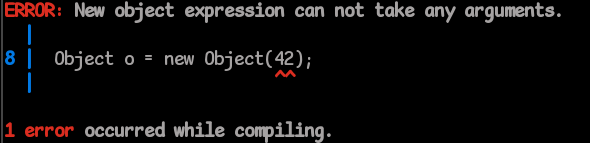
\includegraphics[draft,width=\linewidth,height=5cm]{images/error_message.png}
	\end{figure}
\end{frame}

\begin{frame}{Middle End}
	\begin{columns}
		\begin{column}{0.5\linewidth}
			\begin{itemize}
				\item Constant Folding
				\item Misc. Arithmetic Simplifications
				\item Loop invariant code motion
			\end{itemize}%
			
			\begin{figure}
				\centering
				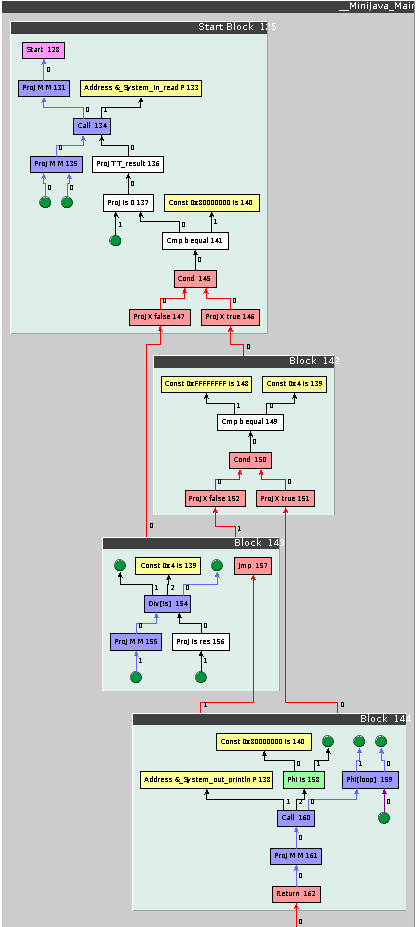
\includegraphics[draft,width=\linewidth,height=4cm]{images/optimization-before.png}
			\end{figure}
		\end{column}
		\begin{column}{0.5\linewidth}
			\begin{itemize}
				\item Common Subexpression Elimination (CSE)
				\item Function Inlining
				\item (Load/Store optimization)
			\end{itemize}
		
			\begin{figure}
				\centering
				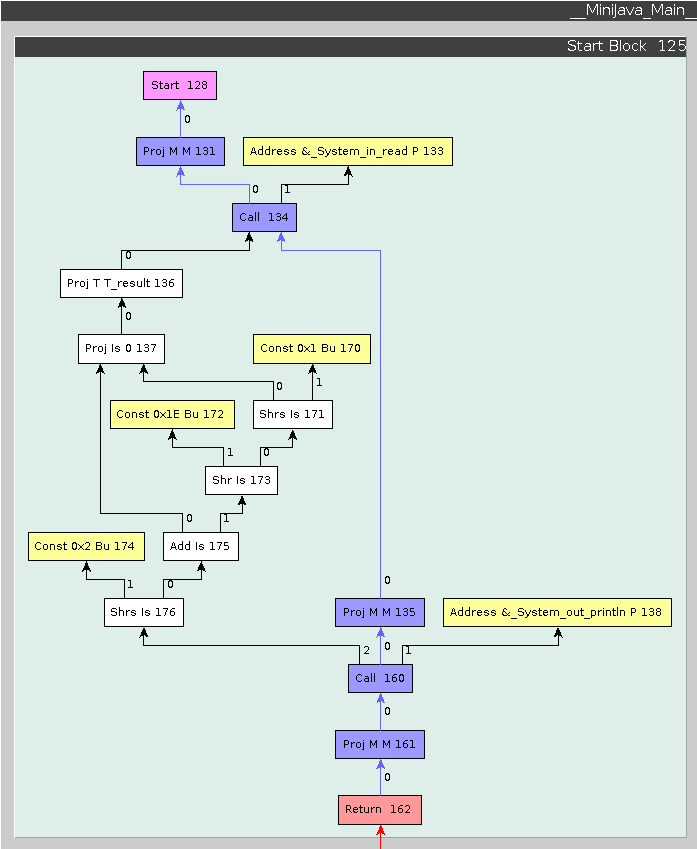
\includegraphics[draft,width=\linewidth,height=4cm]{images/optimization-after.png}
			\end{figure}
		\end{column}
	\end{columns}
\end{frame}

\begin{frame}{Back End - Overview}
	\begin{tikzpicture}[remember picture,overlay,shift=(current page.north west)]
		
	\end{tikzpicture}
\end{frame}

\begin{frame}{Back End - LLIR}
	\framesubtitle{Low-Level Intermediate Representation}
	
	\begin{itemize}
		\item Graph-based
		\item Nodes represent x86 instructions
	\end{itemize}

	\begin{figure}
		\centering
		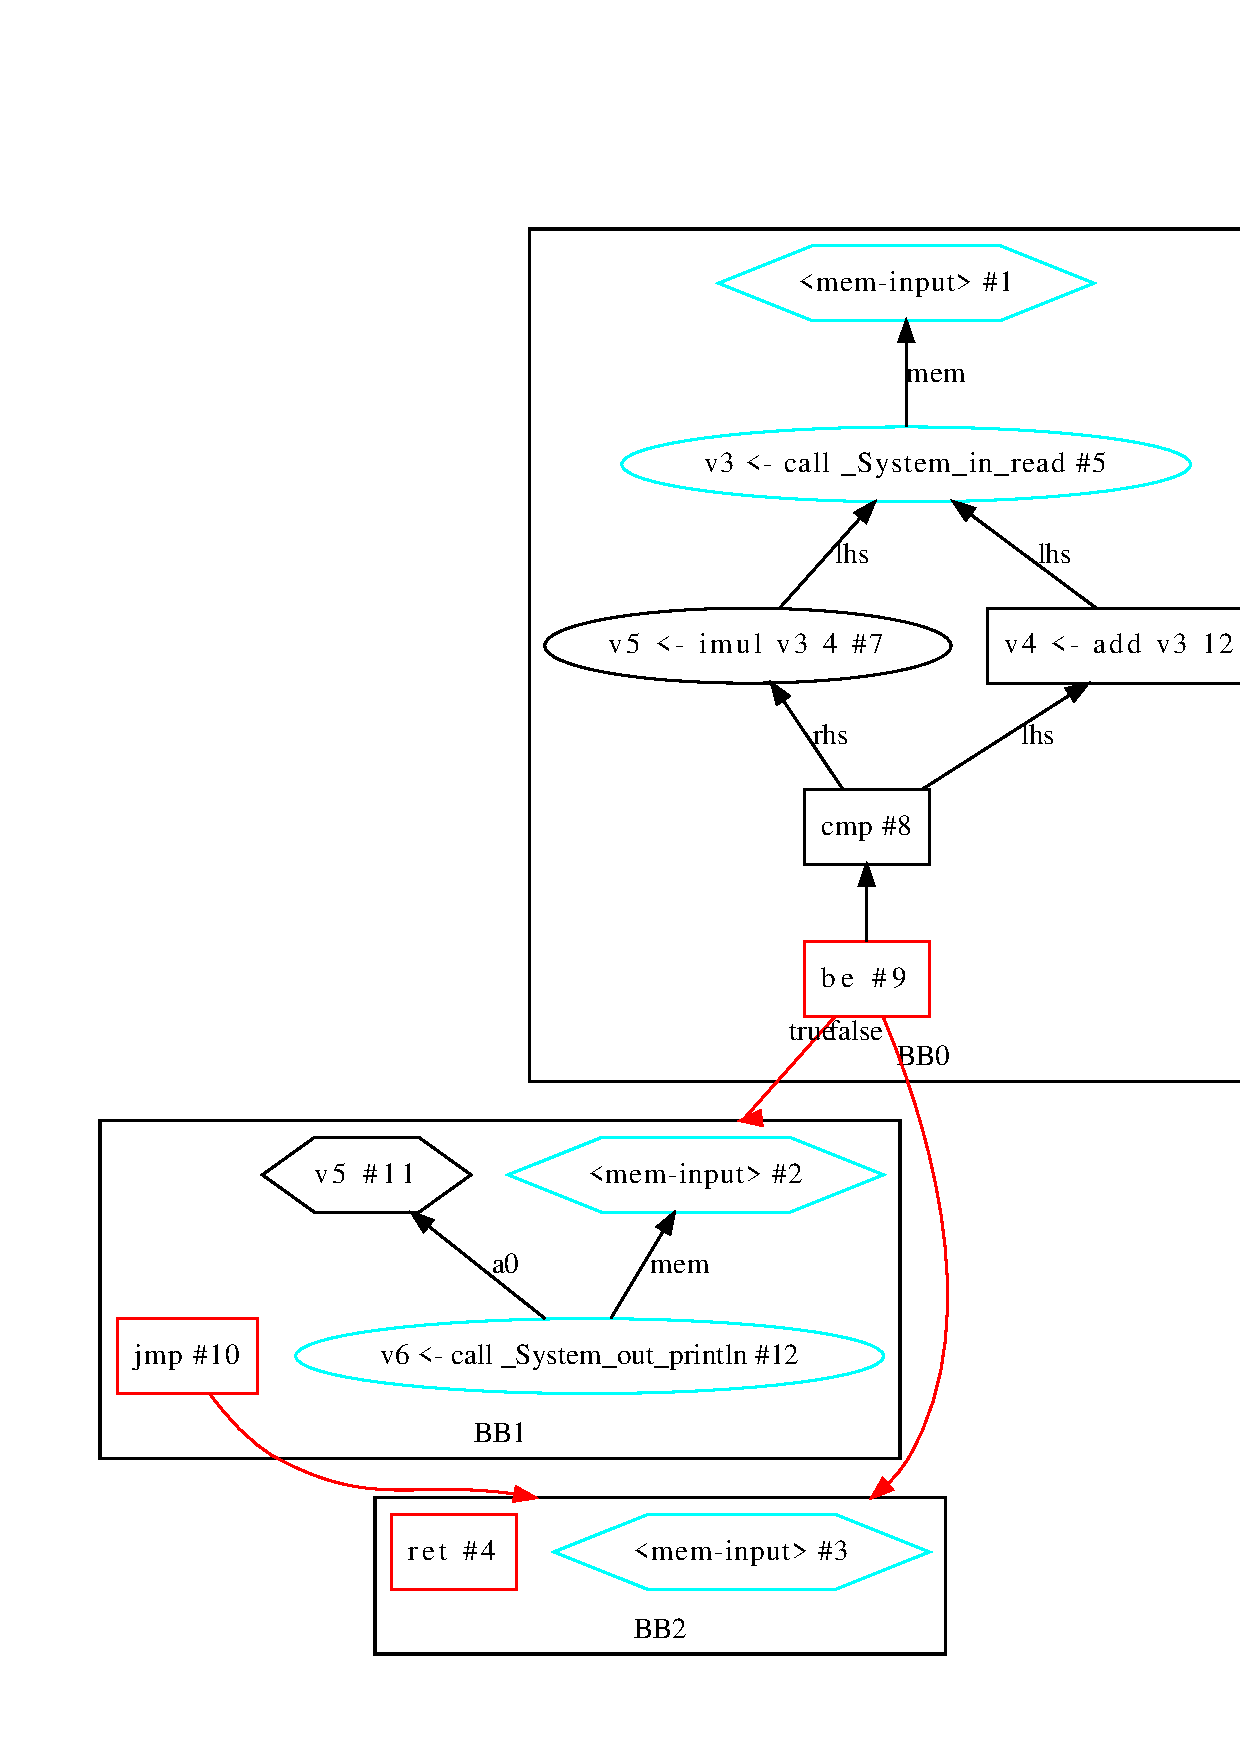
\includegraphics[draft,width=\linewidth,height=5cm]{images/llir-example.png}
	\end{figure}
\end{frame}

\begin{frame}{Back End - SIR}
	\framesubtitle{Scheduled Intermediate Representation}
	
	\begin{itemize}
		\item Includes scheduling information
		\item Modified by peephole optimizer
	\end{itemize}
	
	\begin{figure}
		\centering
		\includegraphics[draft,width=\linewidth,height=5cm]{images/sir-example.png}
	\end{figure}
	
\end{frame}

\begin{frame}{Back End - SIR}
	\framesubtitle{Scheduled Intermediate Representation}
	
	\begin{figure}
		\centering
		\includegraphics[draft,width=\linewidth,height=0.7\textheight]{images/sir-example.png}
	\end{figure}
	
\end{frame}

\appendix
\beginbackup

\begin{frame}{References}
\printbibliography
\end{frame}


\backupend

\end{document}
